\documentclass{ximera}
 

\usepackage{epsfig}

\graphicspath{
  {./}
  {figures/}
}

\usepackage{morewrites}
\makeatletter
\newcommand\subfile[1]{%
\renewcommand{\input}[1]{}%
\begingroup\skip@preamble\otherinput{#1}\endgroup\par\vspace{\topsep}
\let\input\otherinput}
\makeatother

\newcommand{\includeexercises}{\directlua{dofile("/home/jim/linearAlgebra/laode/exercises.lua")}}

%\newcounter{ccounter}
%\setcounter{ccounter}{1}
%\newcommand{\Chapter}[1]{\setcounter{chapter}{\arabic{ccounter}}\chapter{#1}\addtocounter{ccounter}{1}}

%\newcommand{\section}[1]{\section{#1}\setcounter{thm}{0}\setcounter{equation}{0}}

%\renewcommand{\theequation}{\arabic{chapter}.\arabic{section}.\arabic{equation}}
%\renewcommand{\thefigure}{\arabic{chapter}.\arabic{figure}}
%\renewcommand{\thetable}{\arabic{chapter}.\arabic{table}}

%\newcommand{\Sec}[2]{\section{#1}\markright{\arabic{ccounter}.\arabic{section}.#2}\setcounter{equation}{0}\setcounter{thm}{0}\setcounter{figure}{0}}

\newcommand{\Sec}[2]{\section{#1}}

\setcounter{secnumdepth}{2}
%\setcounter{secnumdepth}{1} 

%\newcounter{THM}
%\renewcommand{\theTHM}{\arabic{chapter}.\arabic{section}}

\newcommand{\trademark}{{R\!\!\!\!\!\bigcirc}}
%\newtheorem{exercise}{}

\newcommand{\dfield}{{\sf dfield9}}
\newcommand{\pplane}{{\sf pplane9}}

\newcommand{\EXER}{\section*{Exercises}}%\vspace*{0.2in}\hrule\small\setcounter{exercise}{0}}
\newcommand{\CEXER}{}%\vspace{0.08in}\begin{center}Computer Exercises\end{center}}
\newcommand{\TEXER}{} %\vspace{0.08in}\begin{center}Hand Exercises\end{center}}
\newcommand{\AEXER}{} %\vspace{0.08in}\begin{center}Hand Exercises\end{center}}

% BADBAD: \newcommand{\Bbb}{\bf}

\newcommand{\R}{\mbox{$\Bbb{R}$}}
\newcommand{\C}{\mbox{$\Bbb{C}$}}
\newcommand{\Z}{\mbox{$\Bbb{Z}$}}
\newcommand{\N}{\mbox{$\Bbb{N}$}}
\newcommand{\D}{\mbox{{\bf D}}}
\usepackage{amssymb}
%\newcommand{\qed}{\hfill\mbox{\raggedright$\square$} \vspace{1ex}}
%\newcommand{\proof}{\noindent {\bf Proof:} \hspace{0.1in}}

\newcommand{\setmin}{\;\mbox{--}\;}
\newcommand{\Matlab}{{M\small{AT\-LAB}} }
\newcommand{\Matlabp}{{M\small{AT\-LAB}}}
\newcommand{\computer}{\Matlab Instructions}
\newcommand{\half}{\mbox{$\frac{1}{2}$}}
\newcommand{\compose}{\raisebox{.15ex}{\mbox{{\scriptsize$\circ$}}}}
\newcommand{\AND}{\quad\mbox{and}\quad}
\newcommand{\vect}[2]{\left(\begin{array}{c} #1_1 \\ \vdots \\
 #1_{#2}\end{array}\right)}
\newcommand{\mattwo}[4]{\left(\begin{array}{rr} #1 & #2\\ #3
&#4\end{array}\right)}
\newcommand{\mattwoc}[4]{\left(\begin{array}{cc} #1 & #2\\ #3
&#4\end{array}\right)}
\newcommand{\vectwo}[2]{\left(\begin{array}{r} #1 \\ #2\end{array}\right)}
\newcommand{\vectwoc}[2]{\left(\begin{array}{c} #1 \\ #2\end{array}\right)}

\newcommand{\ignore}[1]{}


\newcommand{\inv}{^{-1}}
\newcommand{\CC}{{\cal C}}
\newcommand{\CCone}{\CC^1}
\newcommand{\Span}{{\rm span}}
\newcommand{\rank}{{\rm rank}}
\newcommand{\trace}{{\rm tr}}
\newcommand{\RE}{{\rm Re}}
\newcommand{\IM}{{\rm Im}}
\newcommand{\nulls}{{\rm null\;space}}

\newcommand{\dps}{\displaystyle}
\newcommand{\arraystart}{\renewcommand{\arraystretch}{1.8}}
\newcommand{\arrayfinish}{\renewcommand{\arraystretch}{1.2}}
\newcommand{\Start}[1]{\vspace{0.08in}\noindent {\bf Section~\ref{#1}}}
\newcommand{\exer}[1]{\noindent {\bf \ref{#1}}}
\newcommand{\ans}{}
\newcommand{\matthree}[9]{\left(\begin{array}{rrr} #1 & #2 & #3 \\ #4 & #5 & #6
\\ #7 & #8 & #9\end{array}\right)}
\newcommand{\cvectwo}[2]{\left(\begin{array}{c} #1 \\ #2\end{array}\right)}
\newcommand{\cmatthree}[9]{\left(\begin{array}{ccc} #1 & #2 & #3 \\ #4 & #5 &
#6 \\ #7 & #8 & #9\end{array}\right)}
\newcommand{\vecthree}[3]{\left(\begin{array}{r} #1 \\ #2 \\
#3\end{array}\right)}
\newcommand{\cvecthree}[3]{\left(\begin{array}{c} #1 \\ #2 \\
#3\end{array}\right)}
\newcommand{\cmattwo}[4]{\left(\begin{array}{cc} #1 & #2\\ #3
&#4\end{array}\right)}

\newcommand{\Matrix}[1]{\ensuremath{\left(\begin{array}{rrrrrrrrrrrrrrrrrr} #1 \end{array}\right)}}

\newcommand{\Matrixc}[1]{\ensuremath{\left(\begin{array}{cccccccccccc} #1 \end{array}\right)}}



\renewcommand{\labelenumi}{\theenumi)}
\newenvironment{enumeratea}%
{\begingroup
 \renewcommand{\theenumi}{\alph{enumi}}
 \renewcommand{\labelenumi}{(\theenumi)}
 \begin{enumerate}}
 {\end{enumerate}\endgroup}



\newcounter{help}
\renewcommand{\thehelp}{\thesection.\arabic{equation}}

%\newenvironment{equation*}%
%{\renewcommand\endequation{\eqno (\theequation)* $$}%
%   \begin{equation}}%
%   {\end{equation}\renewcommand\endequation{\eqno \@eqnnum
%$$\global\@ignoretrue}}

%\input{psfig.tex}

\author{Martin Golubitsky and Michael Dellnitz}

%\newenvironment{matlabEquation}%
%{\renewcommand\endequation{\eqno (\theequation*) $$}%
%   \begin{equation}}%
%   {\end{equation}\renewcommand\endequation{\eqno \@eqnnum
% $$\global\@ignoretrue}}

\newcommand{\soln}{\textbf{Solution:} }
\newcommand{\exercap}[1]{\centerline{Figure~\ref{#1}}}
\newcommand{\exercaptwo}[1]{\centerline{Figure~\ref{#1}a\hspace{2.1in}
Figure~\ref{#1}b}}
\newcommand{\exercapthree}[1]{\centerline{Figure~\ref{#1}a\hspace{1.2in}
Figure~\ref{#1}b\hspace{1.2in}Figure~\ref{#1}c}}
\newcommand{\para}{\hspace{0.4in}}

\renewenvironment{solution}{\suppress}{\endsuppress}

\ifxake
\newenvironment{matlabEquation}{\begin{equation}}{\end{equation}}
\else
\newenvironment{matlabEquation}%
{\let\oldtheequation\theequation\renewcommand{\theequation}{\oldtheequation*}\begin{equation}}%
  {\end{equation}\let\theequation\oldtheequation}
\fi

\makeatother

\begin{document}
\begin{exercise} \label{c8.2.7}
Consider the system of differential equations \eqref{e:global2exam}
that depends on the constant $a$.  
\begin{itemize}
\item[(a)]	Find the equilibria of this system.
\item[(b)]	Find the Jacobian matrices at the equilibria.  
\item[(c)]	For which values of $a$ are the equilibria not
		hyperbolic?
\item[(d)]	For those values of $a$ where the equilibria are 
		hyperbolic, determine whether or not these equilibria 
		are asymptotically stable.
\item[(e)]	For each nonhyperbolic equilibrium, write the linearized 
		system and draw its phase plane.
\end{itemize}

\begin{solution}

(a) Solving system \eqref{e:global2exam} for $\dot{x} = \dot{y} = 0$
yields equilibria at $(0,0)$, $(\sqrt{2.2},0)$, and $(-\sqrt{2.2},0)$.

(b) The general Jacobian matrix for \eqref{e:global2exam} is
\[
(dJ)_{(x,y)} = \cmattwo{0}{1}{2.2 - 3x^2 + ay}{2.1 + ax}.
\]
The Jacobian matrices at the equilibria are:
\[ \begin{array}{rcl}
(dJ)_{(0,0)} & = & \cmattwo{0}{1}{2.2}{2.1} \\
(dJ)_{(\sqrt{2.2},0)} & = & \cmattwo{0}{1}{-4.4}{2.1 + \sqrt{2.2}a} \\
(dJ)_{(-\sqrt{2.2},0)} & = & \cmattwo{0}{1}{-4.4}{2.1 - \sqrt{2.2}a}. \\
\end{array}
\]

(c) \ans The Jacobian of the equilibrium at $(\sqrt{2.2},0)$ is not
hyperbolic at $a = -2.1\left/\sqrt{2.2}\right.$, and the Jacobian of the
equilibrium at $(-\sqrt{2.2},0)$ is not hyperbolic at
$a = 2.1\left/\sqrt{2.2}\right.$.

\soln Note that a matrix is nonhyperbolic if the determinant is positive
and the trace is zero.

(d) \ans The equilibrium at $(\sqrt{2.2},0)$ is asymptotically stable for
$a < -2.1\left/\sqrt{2.2}\right.$ and the equilibrium at
$(-\sqrt{2.2},0)$ is asymptotically stable for
$a > 2.1\left/\sqrt{2.2}\right.$.  Thus, there is no value of $a$ for which
both equilibria are stable.  The equilibrium at $(0,0)$ is not stable,
since the eigenvalues of the Jacobian have opposite sign.

\soln Note that the determinant of the Jacobian is always positive, so
the equilibria are stable for values of $a$ at which the trace is negative.

(e) For $a = -2.1/\sqrt{2.2}$, the equilibrium at $(\sqrt{2.2},0)$
is non-hyperbolic, with Jacobian matrix
\[
(dJ)_{(\sqrt{2.2},0)} = \mattwo{0}{1}{-4.4}{0}.
\]
The linear system $\dot{X} = (dJ)_{(\sqrt{2.2},0)}X$ is pictured in
Figure~\ref{c8.2.7}.  Note that the system is a center.  For
$a = 2.1/\sqrt{2.2}$, the equilibrium at $(-\sqrt{2.2},0)$ is
nonhyperbolic.  Its Jacobian at this point is identical to
$(dJ)_{(\sqrt{2.2},0)}$.

\begin{figure}[htb]
                       \centerline{%
                       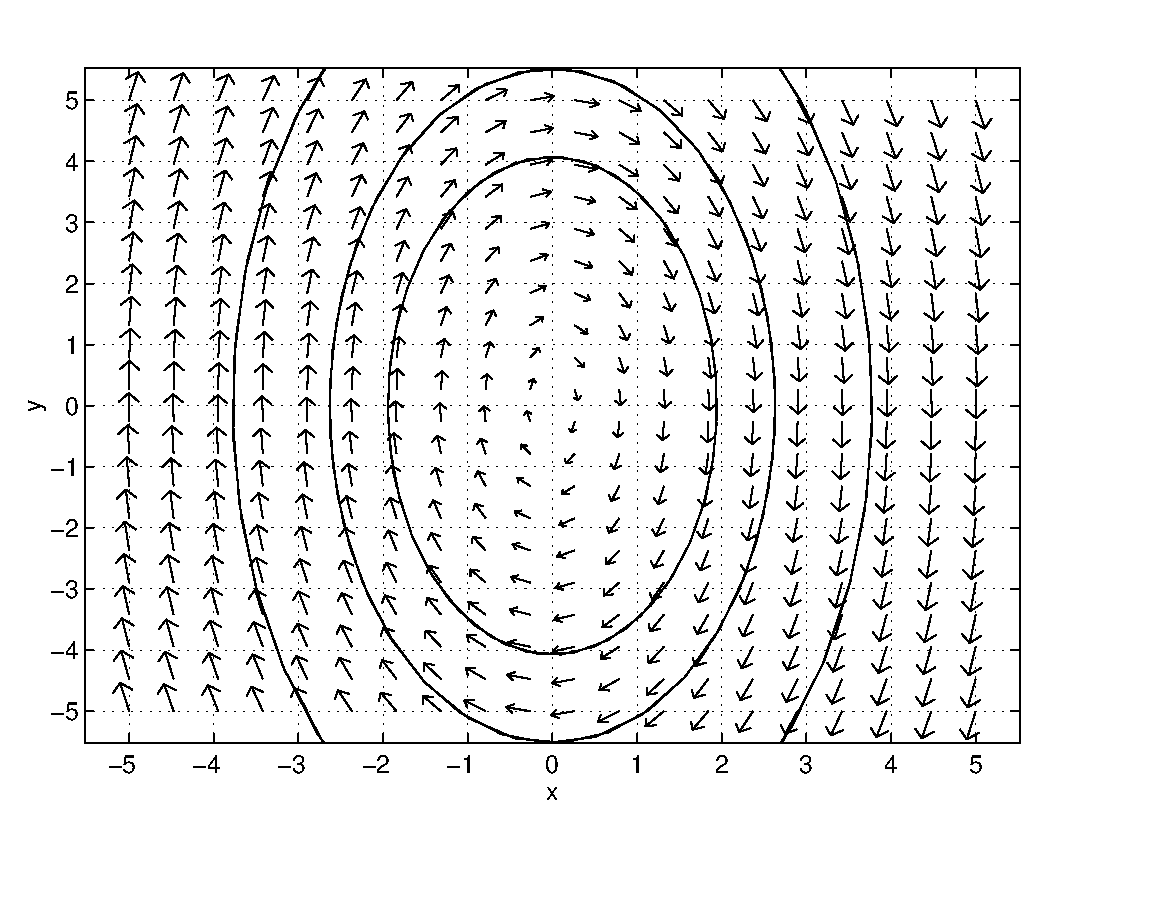
\psfig{file=exfigure/8-2-7.eps,width=3.0in}}
                \exercap{c8.2.7}
\end{figure}

\end{solution}
\end{exercise}
\end{document}
